\documentclass{standalone}
\usepackage{tikz}
\usepackage{pgfplots}
\pgfplotsset{width=32cm,height=18cm,compat=1.3}
\pgfplotsset{every tick label/.append style={font=\Huge}}
\usepackage{filecontents}

\usetikzlibrary{patterns}

\definecolor{citrine}{rgb}{0.89, 0.82, 0.04}

\begin{document}
	\centering
		\vspace{1.5em}
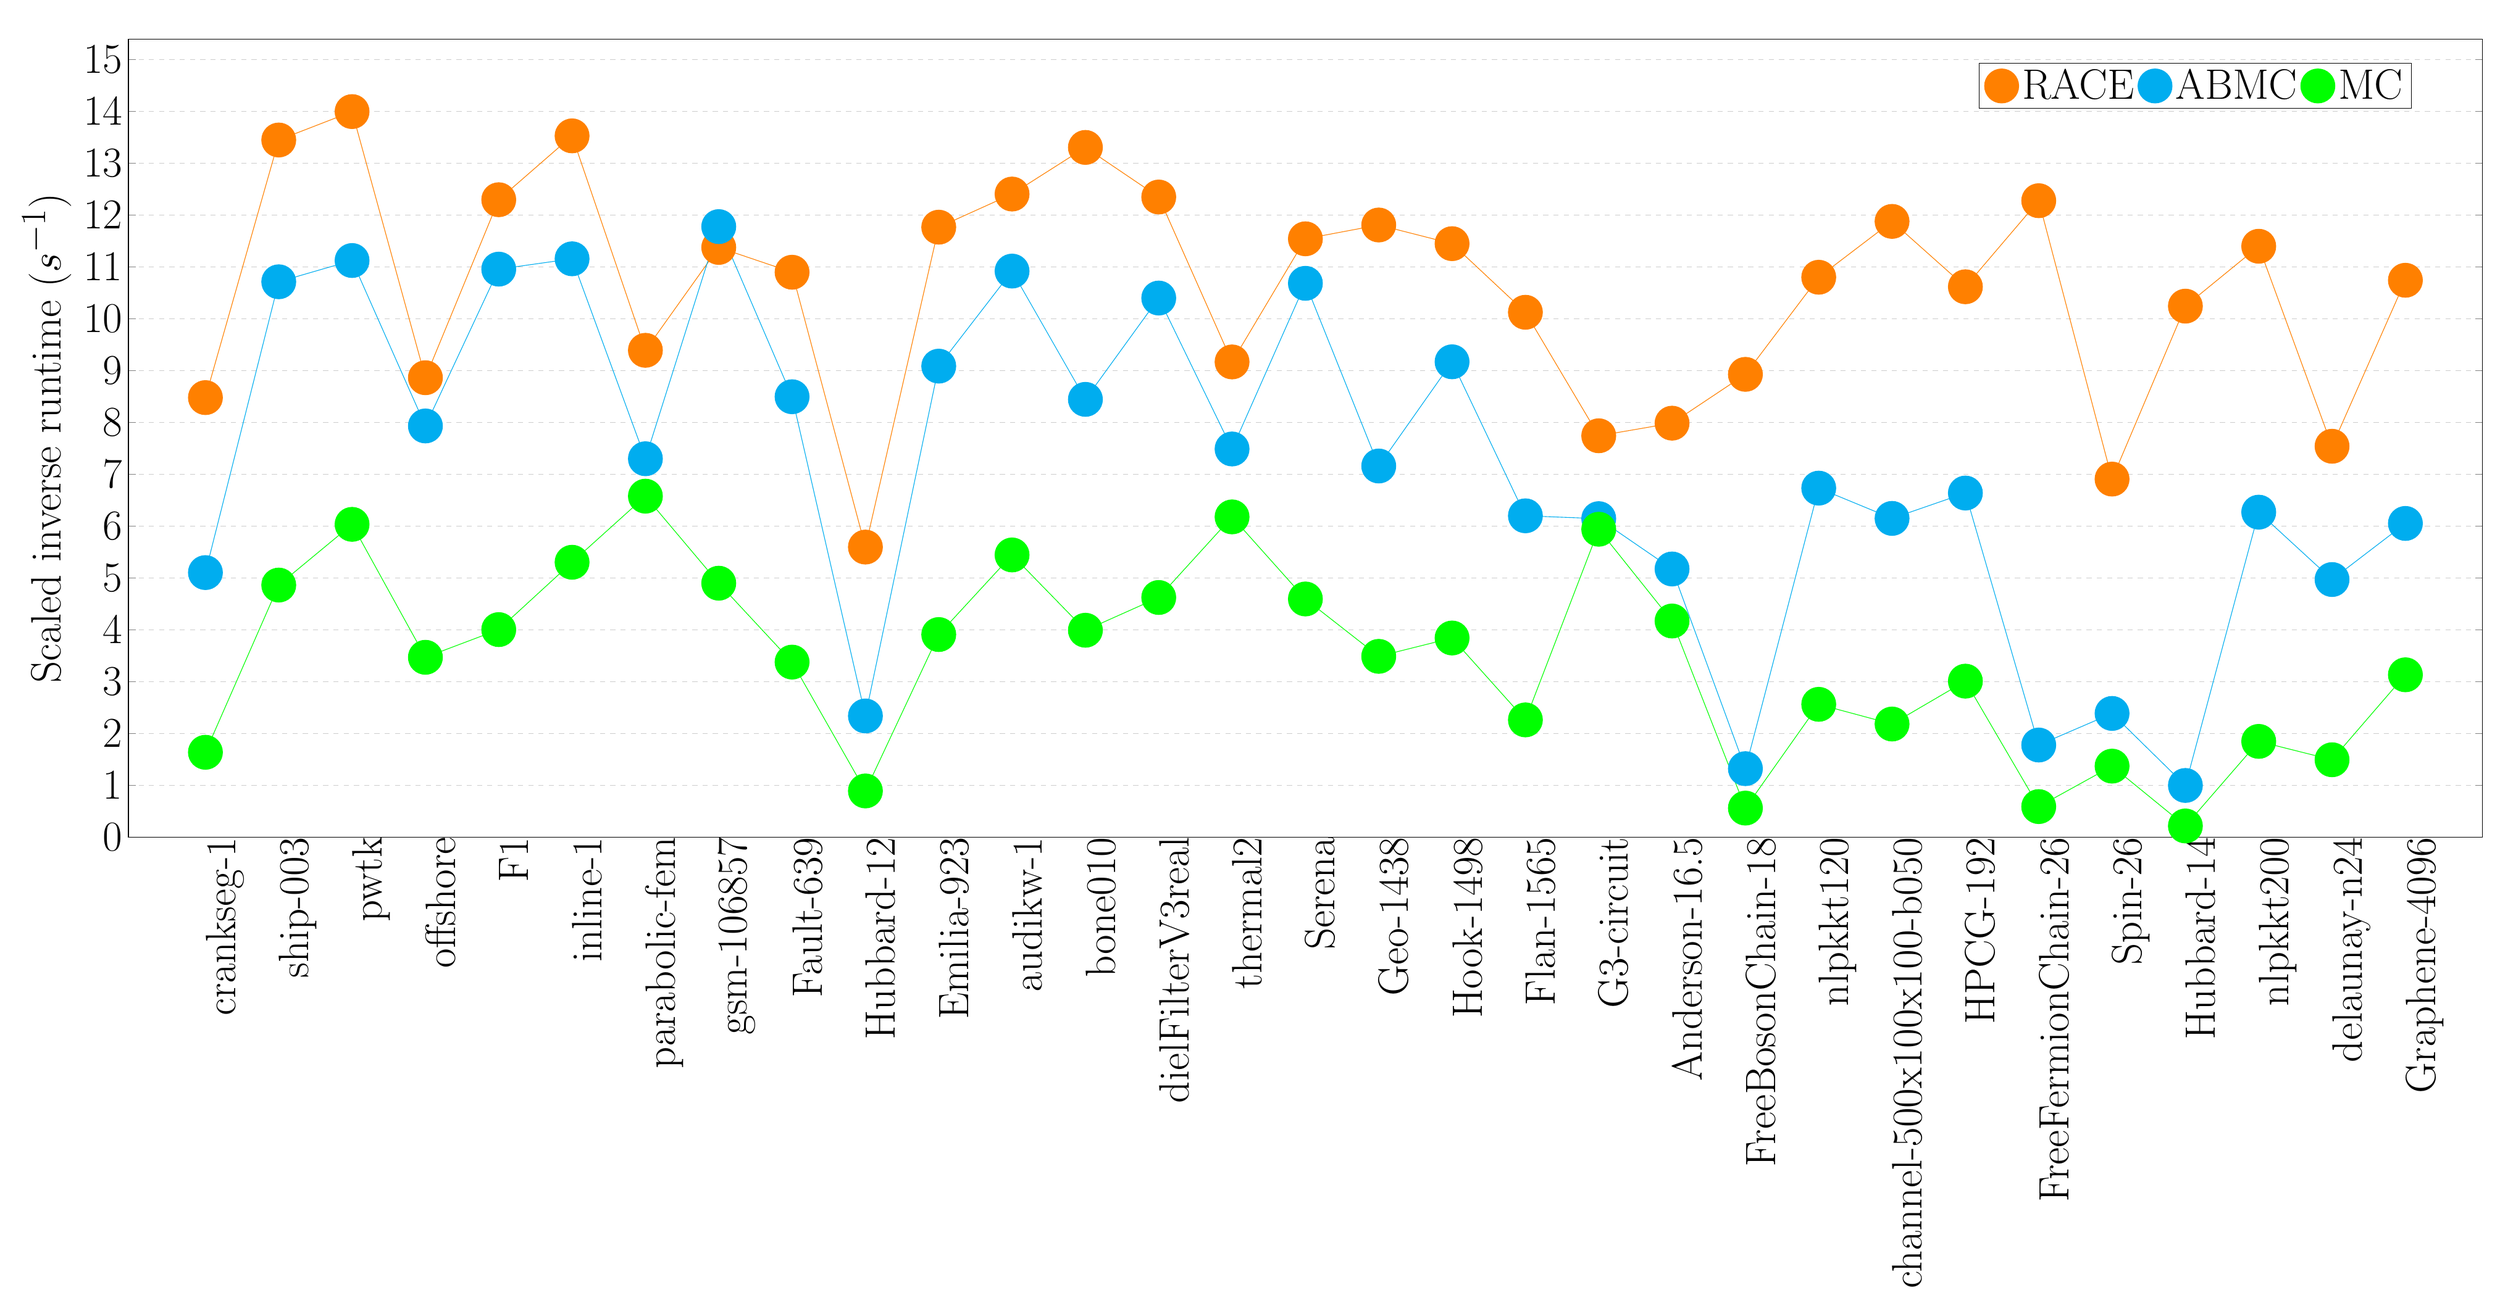
\begin{tikzpicture}
		%	\node at (13.25,15) {\LARGE{}};
			\begin{axis}[
		%	xmin=0.25, xmax=7.25,
			ymin=0, %ymax=3.25,
			xtick={1, 2, 3, 4, 5, 6, 7, 8, 9, 10, 11, 12, 13, 14, 15, 16, 17, 18, 19, 20, 21, 22, 23, 24, 25, 26, 27, 28, 29, 30, 31},
		%	ytick={0,0.5,1,1.5,2,2.5,3},
			xticklabels={crankseg-1, ship-003, pwtk, offshore, F1, inline-1, parabolic-fem, gsm-106857, Fault-639, Hubbard-12, Emilia-923, audikw-1, bone010, dielFilterV3real, thermal2, Serena, Geo-1438, Hook-1498, Flan-1565, G3-circuit, Anderson-16.5, FreeBosonChain-18, nlpkkt120, channel-500x100x100-b050, HPCG-192, FreeFermionChain-26, Spin-26, Hubbard-14, nlpkkt200, delaunay-n24, Graphene-4096},
			width  = 50cm,
			height = 18cm,
			major x tick style = transparent,
			%	minor ytick={1, 5, 10, 15, 20, 25, 30 ,35,40},
			grid = minor,	
			%add_bar_commands
			ymajorgrids = true,
			grid style={dashed, gray!40},
			ylabel = {\Huge{Scaled inverse runtime ($s^{-1}$)}},
		%	symbolic x coords={Graphene-2048-2048, Graphene-4096-4096, Spin-24-24-24},
			x tick label style={rotate=90, anchor=north east, inner sep=0mm, font={\Huge}},
			tick label style={font={\Huge}},
			scaled y ticks = false,
			enlarge x limits=0.035,
			legend cell align=left,
			legend style={font=\Huge},
			legend columns=-1,
			legend style={
				%at={(1,1.05)},
				%anchor=south east,
				%column sep=1ex,
				legend pos=north east
			},
			%spl_legend_code
			title= {\Huge\scalebox{1.5}{{}}}
			]

\addplot[ mark=*, mark size=10pt, mark options={orange}, draw=orange , y filter/.code={\pgfmathparse{\pgfmathresult*1000}\pgfmathresult}] plot coordinates{(1,.00847579519230769230) (2,.01344527352941176470) (3,.01399338725490196078) (4,.00885941844660194174) (5,.01229319306930693069) (6,.01352516500000000000) (7,.00938811553398058252) (8,.01137282700000000000) (9,.01089423302752293577) (10,.00559241466666666666) (11,.01176350560747663551) (12,.01240261584158415841) (13,.01330212277227722772) (14,.01234528514851485148) (15,.00916399504950495049) (16,.01153916767676767676) (17,.01180574313725490196) (18,.01144560776699029126) (19,.01012190977443609022) (20,.00773939223300970873) (21,.00798259909909909909) (22,.00892440967741935483) (23,.01079772079207920792) (24,.01187504705882352941) (25,.01061394272727272727) (26,.01227428333333333333) (27,.00690376209677419354) (28,.01024022839506172839) (29,.01139539509803921568) (30,.00753709509803921568) (31,.01073943960396039603)};
\addplot[ mark=*, mark size=10pt, mark options={cyan}, draw=cyan , y filter/.code={\pgfmathparse{\pgfmathresult*1000}\pgfmathresult}] plot coordinates{(1,.00510026838235294117) (2,.01071030545454545454) (3,.01112031065573770491) (4,.00792886666666666666) (5,.01095415370370370370) (6,.01115330275229357798) (7,.00729625520000000000) (8,.01177436633663366336) (9,.00849239788732394366) (10,.00233437315436241610) (11,.00908274843750000000) (12,.01091645754716981132) (13,.00844184642857142857) (14,.01039645267857142857) (15,.00748486666666666666) (16,.01068056100000000000) (17,.00715630272108843537) (18,.00916648547008547008) (19,.00619546137566137566) (20,.00614078235294117647) (21,.00516998214285714285) (22,.00131771881188118811) (23,.00672954672131147540) (24,.00614530081967213114) (25,.00663471300813008130) (26,.00177355357142857142) (27,.00238312982456140350) (28,.00099383696498054474) (29,.00626595645161290322) (30,.00496627758620689655) (31,.00604842518518518518)};
\addplot[ mark=*, mark size=10pt, mark options={green}, draw=green , y filter/.code={\pgfmathparse{\pgfmathresult*1000}\pgfmathresult}] plot coordinates{(1,.00163344173228346456) (2,.00485936106194690265) (3,.00603067520661157024) (4,.00346590166666666666) (5,.00400048320000000000) (6,.00529947623762376237) (7,.00657436363636363636) (8,.00489530909090909090) (9,.00337343496932515337) (10,.00088796991525423728) (11,.00390503673469387755) (12,.00544043434343434343) (13,.00398789814814814814) (14,.00461983412698412698) (15,.00617466911764705882) (16,.00459114601769911504) (17,.00348426100628930817) (18,.00383847183098591549) (19,.00225848768115942028) (20,.00593624958677685950) (21,.00416610916030534351) (22,.00055689095238095238) (23,.00255869469696969696) (24,.00217879928057553956) (25,.00300603897058823529) (26,.00058601413427561837) (27,.00136656821705426356) (28,.00021239850000000000) (29,.00184372313432835820) (30,.00148933987341772151) (31,.00312860137931034482)};
	%addplot cmd

	\legend{RACE, ABMC, MC}

	\end{axis}			
\end{tikzpicture}

\end{document}

